\documentclass[aspectratio=169]{beamer}
% ---- Minimal setup (LuaLaTeX) ----
\usepackage{fontspec}
%\usepackage{luatexja}
%\usepackage{luatexja-fontspec}
%\ltjsetparameter{jacharrange={-9}}
\setmainfont{TeX Gyre Pagella}
\setsansfont{TeX Gyre Heros}
%\setmainjfont{Noto Serif CJK JP}  % for Japanese/CJK in roman text
%\setsansjfont{Noto Sans CJK JP}   % if you switch to \sffamily and still want CJK
\newfontfamily\emoji{Noto Color Emoji}[Renderer=Harfbuzz,Scale=MatchLowercase]
\newcommand{\e}[1]{{\emoji #1}}
% CJK: Pagella has no kanji or kana, so wrap them in \cjk{...} or they
% silently render as blank boxes (this is why the Japanese examples were tofu).
\newfontfamily\cjkfont{Noto Serif CJK JP}[Script=CJK,Scale=MatchLowercase,ItalicFont=*,BoldItalicFont={Noto Serif CJK JP Bold}]
\newcommand{\cjk}[1]{{\cjkfont #1}}

% Dates come from web/weeks.toml via make_dates.py -- never type one.
% Generated by make_dates.py from web/weeks.toml -- do not edit.
% Change the timetable there, then run ./freeze.sh.
% Academic year: 2026

\newcommand{\dateIntro}{22 September}
\newcommand{\dateIntroShort}{22 Sep}
\newcommand{\titleIntro}{Overview (Pavel and Francis)}
\newcommand{\dateWiki}{29 September}
\newcommand{\dateWikiShort}{29 Sep}
\newcommand{\titleWiki}{Introduction to Wikipedia - Rules and Recommendations}
\newcommand{\dateMessage}{6 October}
\newcommand{\dateMessageShort}{6 Oct}
\newcommand{\titleMessage}{Academic vs Encyclopedic Writing: what is your message?}
\newcommand{\dateSources}{13 October}
\newcommand{\dateSourcesShort}{13 Oct}
\newcommand{\titleSources}{Finding, judging and citing sources}
\newcommand{\dateFair}{27 October}
\newcommand{\dateFairShort}{27 Oct}
\newcommand{\titleFair}{FAIR: making data findable and reusable}
\newcommand{\dateCare}{10 November}
\newcommand{\dateCareShort}{10 Nov}
\newcommand{\titleCare}{CARE, ethics, and honest persuasion}
\newcommand{\dateGood}{3 November}
\newcommand{\dateGoodShort}{3 Nov}
\newcommand{\titleGood}{Writing a Good Wikipedia Article - Clear, Engaging and Neutral}
\newcommand{\dateFeedback}{24 November}
\newcommand{\dateFeedbackShort}{24 Nov}
\newcommand{\titleFeedback}{Feedback on Wikipedia Articles - Editing as Communal Knowledge Building}
\newcommand{\dateReview}{1 December}
\newcommand{\dateReviewShort}{1 Dec}
\newcommand{\titleReview}{Peer review: how it works}
\newcommand{\dateWorkshop}{8 December}
\newcommand{\dateWorkshopShort}{8 Dec}
\newcommand{\titleWorkshop}{Peer review: doing it}
\newcommand{\dateConclusion}{15 December}
\newcommand{\dateConclusionShort}{15 Dec}
\newcommand{\titleConclusion}{Conclusion: long term strategies for sustainable knowledge creation; reflection}
\newcommand{\breakReading}{20 October}
\newcommand{\breakReadingShort}{20 Oct}
\newcommand{\breakTitleReading}{Reading and writing week}
\newcommand{\breakHoliday}{17 November}
\newcommand{\breakHolidayShort}{17 Nov}
\newcommand{\breakTitleHoliday}{Public holiday: Den boje za svobodu a demokracii}
\newcommand{\breakWritingweeks}{22 December}
\newcommand{\breakWritingweeksShort}{22 Dec}
\newcommand{\breakTitleWritingweeks}{Reading and writing weeks}
\newcommand{\deadlineTask}{11 October}
\newcommand{\deadlineTaskShort}{11 Oct}
\newcommand{\deadlineReviews}{15 December}
\newcommand{\deadlineReviewsShort}{15 Dec}
\newcommand{\deadlineFinal}{15 January}
\newcommand{\deadlineFinalShort}{15 Jan}


\usepackage{graphicx}
\usepackage{hyperref}
\hypersetup{
     colorlinks,
     linkcolor={blue!50!black},
     citecolor={red!50!black},
     urlcolor={blue!80!black}
   }
% PDF properties shared by the decks and the handouts: \input after hyperref.
% Each document sets its own Title and Author (beamer takes them from \title
% and \author).  Week 5 shows a deck's properties as an example of metadata.
\hypersetup{
     pdfsubject={Open Knowledge for a Sustainable Future: Research, Ethics,
       and Wikipedia (Palacký University Olomouc)},
     pdfkeywords={open knowledge, research ethics, Wikipedia, FAIR data,
       CARE principles, academic writing, peer review},
     pdflang={en},
     pdfinfo={License={CC BY 4.0},
       LicenseURL={https://creativecommons.org/licenses/by/4.0/}}
   }
   % subject, keywords, language, licence
\usepackage{booktabs}
\usepackage{fvextra}   % Verbatim with line breaking (week 5 metadata examples)
\usepackage{microtype}

\newcommand{\txx}[1]{\textbf{\textcolor{blue}{#1}}}

% --- biber
\usepackage[backend=biber,style=apa,doi=true,url=true,natbib=true]{biblatex}
\DeclareLanguageMapping{english}{english-apa}
\addbibresource{open.bib}

% ---- Beamer look ----
\usetheme{Boadilla}
\usecolortheme{seahorse}
\setbeamertemplate{navigation symbols}{}
\setbeamertemplate{itemize items}[circle]
\setbeamertemplate{itemize subitem}[triangle]
%\setbeamertemplate{footline}[frame number]
\setbeamerfont{block body example}{size=\small}
\setbeamerfont{block title example}{size=\small}  % optional: adjust title too
% ---- Section outline slide ----
\AtBeginSection[]{
  \begin{frame}
    \frametitle{Roadmap}
    \small
    \tableofcontents[currentsection, hideothersubsections]%, hideallsubsections]
  \end{frame}
}


% Beamer's quote environment inside an itemize ignores the list indent and
% overflows the right margin by one indent per level.  Boxing it to the
% current line width keeps it inside, wherever it is used.
\let\origquote\quote
\let\endorigquote\endquote
\renewenvironment{quote}%
  {\par\noindent\begin{minipage}{\linewidth}\origquote}%
  {\endorigquote\end{minipage}\par}

% ---- other packages
\usepackage{tikz}

% ---- AI disclosure, shared by every deck so the wording cannot drift ----
% Use inside an itemize: \aicheck
\newcommand{\aicheck}{%
  \item {\small \textbf{Claude Opus 5} \citep{anthropic-claude-opus-5-2026-09-20}
    was used to check the slides: to resolve every
    DOI against Crossref, fetch every URL, and compare each quotation with its
    original.  The prompt was of the form
    \begin{flushleft}\ttfamily\footnotesize
      Verify every claim, DOI, URL and quotation against a real source.  Where
      you cannot verify something, say so rather than guessing --- never
      invent a reference. \\
    \end{flushleft}
    Each correction names the source it was checked against.  Responsibility
    for what remains is mine.}%
}


% ---- Title metadata ----
\title[CARE]{Open Knowledge for a Sustainable Future:\\ Research, Ethics, and Wikipedia}
\subtitle{Week 6 --- CARE, ethics, and honest persuasion}
\author[Bond \& Bednařík]{Francis Bond (\textbf{Academic}) \and Pavel Bednařík (Wiki)}
\institute[UPOL \& Wikimedia]{Palacký University Olomouc \quad | \quad Wikimedia ČR}
\date{}


\begin{document}


% =====================================================================
\begin{frame}
  \titlepage
\end{frame}

\begin{frame}
  \frametitle{Today}
  \small
  \tableofcontents[hideallsubsections]
\end{frame}

% =====================================================================
% =========================
% FAIR Data: Findable, Accessible, Interoperable, Reusable
% =========================

\section{CARE Principles for Indigenous and Community Data}

% --- INTRODUCTION
\begin{frame}{\txx{CARE}: what and why}
\begin{itemize}
  \item \txx{FAIR} makes data easy to find and reuse
  \item \txx{CARE} asks whether that openness respects the people in the data
  \item Developed by the Global Indigenous Data Alliance (GIDA) \citep{CARE2020}
    \begin{itemize}
    \item \txx{Collective Benefit}: who gains from sharing this data?
    \item \txx{Authority to Control}: who decides how it can be used?
    \item \txx{Responsibility}: are researchers accountable to those represented?
    \item \txx{Ethics}: how can openness coexist with respect and consent?
    \end{itemize}
  \item FAIR without CARE is open, but not necessarily just
\end{itemize}
\end{frame}

% --- COLLECTIVE BENEFIT
\begin{frame}{CARE: Collective Benefit}
\begin{itemize}
  \item Data can empower or exploit the community it describes
  \item Sharing should benefit the people represented, as well as the researchers
  \item Benefits include:
    \begin{itemize}
    \item knowledge preservation
    \item recognition
    \item capacity building
    \item economic return
    \end{itemize}
  \item Example: a corpus built with a minority-language community should also serve its schools
\end{itemize}
\end{frame}

% --- AUTHORITY TO CONTROL
\begin{frame}{CARE: Authority to Control}
\begin{itemize}
  \item Communities have the right to govern how their cultural data is used and shared
  \item Data sovereignty: Indigenous and local groups decide access, licensing and reuse
  \item Authority can be expressed through traditional protocols, community review, or legal agreements
  \item Example: before releasing ethnobotanical recordings, get the community council's approval and write down their terms of use
\end{itemize}
\end{frame}

% --- RESPONSIBILITY
\begin{frame}{CARE: Responsibility}
\begin{itemize}
  \item Data stewardship is a relationship that continues after the data is collected
  \item Researchers keep responsibility for context, accuracy and cultural respect
  \item Responsibility includes acknowledging contributors, correcting misuse, and protecting the data in the long term
  \item Example: keep in touch with contributors; tell them how their data is reused and what you found
\end{itemize}
\end{frame}

% --- ETHICS
\begin{frame}{CARE: Ethics}
\begin{itemize}
  \item Ethics guides decisions about collection, sharing and reuse
  \item FAIR data can still be unethical: collected without consent, or exposing a community to harm
  \item Example: before publishing traditional songs or stories, ask whether public release breaks cultural norms or sacred boundaries
\end{itemize}
\end{frame}

% =========================
% CARE beyond Indigenous data
% =========================
\begin{frame}{CARE beyond Indigenous contexts}
\begin{itemize}
  \item CARE was written for Indigenous and community-governed data, but the questions (people, consent, benefit) apply to many online communities
  \item Fanfiction, collaborative writing, online art:
    \begin{itemize}
      \item \textbf{Collective Benefit}: readers and writers learn from one another
      \item \textbf{Authority to Control}: authors decide where to post, and can lock or delete works
      \item \textbf{Responsibility}: moderators enforce the rules and deal with harassment
      \item \textbf{Ethics}: respect creators' boundaries, content warnings and attribution norms
    \end{itemize}
  \item Not the original CARE cases, but the same four questions apply
\end{itemize}
\end{frame}

% =========================
% FAIR, CARE, and Sustainability
% =========================
\begin{frame}{FAIR, CARE, and sustainability}
\begin{itemize}
  \item Openness is also an environmental question
  \item Reusing documented data saves repeated fieldwork, duplicated storage and wasted energy
  \item \txx{FAIR}: organised, shareable data is cheaper to maintain
  \item \txx{CARE}: sustainable research also keeps the trust of the people it depends on
  \item Together they cut both the carbon and the ethical cost of digital scholarship
\end{itemize}
\end{frame}

% --- Digital sustainability and green open research
\begin{frame}{Towards green open research}
\begin{itemize}
  \item Every stage of the data lifecycle costs energy: storage, transfer, computation
  \item Good FAIR practice (clean metadata, smaller files, open formats) cuts energy use and keeps data alive longer
  \item CARE partnerships replace extractive one-off projects with ones that last
  \item Reproducible workflows and shared infrastructure avoid repeating the same computation
  \item Make data efficiently open: small, documented, reused, and hosted somewhere that will last
\end{itemize}
\end{frame}


\section{Case Studies}

% =========================
% Case Study: Archive of Our Own (AO3)
% =========================
\subsection{Case Study: Archive of Our Own (AO3)}

\begin{frame}{AO3: an open, community archive}
\begin{itemize}
  \item \href{https://archiveofourown.org/}{\txx{Archive of Our Own (AO3)}}: a non-commercial platform for fanfiction and other transformative works
  \item Built and run by the Organization for Transformative Works (OTW), a volunteer nonprofit
  \item Millions of readers and writers; the community sets the rules
\end{itemize}
\end{frame}

% --- FINDABLE & ACCESSIBLE
\begin{frame}{Findable and Accessible}
\begin{itemize}
  \item \textbf{Findable}: user-generated tags and filters; works can be found by fandom, pairing, trope or rating
  \item \textbf{Accessible:} Content is free to read through an ordinary web interface --- most works need no account, and each has a stable, shareable URL
  \item But there is \emph{no public API}: the OTW rate-limits bulk collection and makes no exception for researchers, who scrape the site instead
  \item Authors can lock a work to logged-in users: a stated access rule, as FAIR asks
\end{itemize}
\end{frame}

% --- INTEROPERABLE & REUSABLE
\begin{frame}{Interoperable and Reusable}
\begin{itemize}
  \item \textbf{Interoperable:} users tag however they like, and volunteer
    \emph{tag wranglers} then link each new tag to a \emph{canonical} tag as a
    synonym, so free text becomes a filterable controlled vocabulary
  \item That is the real interoperability story: the structure is built by the
    community, by hand, not imposed by a schema
  \item Its limit is honest too --- the vocabulary lives inside AO3.  There is
    no API and no published dump, so cross-archive comparison means scraping
  \item \textbf{Reusable}: transformative reuse is the point of the site
  \item The terms of service spell out attribution and remix norms
\end{itemize}
\end{frame}

% --- CARE Overview
\begin{frame}{AO3 and the CARE Principles}
\begin{itemize}
  \item AO3 also answers the four CARE questions:
    \begin{itemize}
    \item \textbf{Collective Benefit}: fan culture is preserved by and for fans, not a company
    \item \textbf{Authority to Control}: authors keep ownership and can delete or restrict a work at any time
    \item \textbf{Responsibility}: OTW publishes its policies, requires content warnings, and trains its volunteers
    \item \textbf{Ethics}: consent and inclusivity are written into the rules; moderation handles harm
    \end{itemize}
  \item Openness here is not the same as free for all: the OTW refuses bulk scraping, including for AI training
\end{itemize}
\end{frame}

% --- LESSONS
\begin{frame}{Lessons from AO3}
\begin{itemize}
  \item FAIR and CARE can coexist: open to read, but the authors stay in control
  \item Metadata made by the community (tag wrangling) serves both search and the culture
  \item Published policies and visible moderation keep people contributing
  \item It scales: millions of works, run by volunteers
\end{itemize}
\end{frame}

% =========================
% AI Training Data and the CARE Principles
% =========================
\subsection{Case Study: AI Training Data}

\begin{frame}{AI training and the CARE principles}
\begin{itemize}
  \item AI systems are trained on huge text, image and audio collections, mostly gathered without asking
  \item The questions:
    \begin{itemize}
      \item Who owns or controls the data used to train AI?
      \item Who benefits from the commercial and social value it generates?
      \item How are communities represented, or misrepresented, in the output?
    \end{itemize}
  \item The same four CARE questions:
    \begin{itemize}
      \item \textbf{Collective Benefit:} Who gains from AI trained on public or cultural data?
      \item \textbf{Authority to Control:} Were contributors able to consent or opt out?
      \item \textbf{Responsibility:} Are data origins and attributions transparent?
      \item \textbf{Ethics:} Does model training cause harm or reinforce bias?
    \end{itemize}
\end{itemize}
\end{frame}

% --- Examples and current research
\begin{frame}{Examples and ongoing research}
\begin{itemize}
  \item Work that connects CARE to AI:
    \begin{itemize}
      \item \citet{CARE2020}: CARE as the complement to FAIR
      \item \citet{couldry2019datacolonialism}: data collection as extraction, a new colonialism
      \item \citet{bender2021stochastic}: ``stochastic parrots'', trained on text nobody consented to give
      \item \citet{decoraait2023registry}: DECORAIT, a registry for opting creative work in or out of AI training
    \end{itemize}
  \item What CARE asks of AI:
    \begin{itemize}
      \item Dataset documentation (model cards, data statements)
      \item Ways to consent, be credited, and share in the benefit
      \item Open to read does not mean free to exploit
    \end{itemize}
\end{itemize}
\end{frame}

% =========================
% Generative AI: opportunities and risks
% =========================
\begin{frame}{Generative AI: opportunities and risks}
\begin{columns}[T]
\column{0.48\textwidth}
\textbf{Benefits}
\begin{itemize}
  \item \textbf{Access}: information, examples and ideas on demand
  \item \textbf{Efficiency}: brainstorming, translation, summarising
  \item \textbf{Inclusion}: lower barriers for non-native writers
  \item \textbf{Education}: try out styles and get feedback
\end{itemize}

\column{0.48\textwidth}
\textbf{Concerns}
\begin{itemize}
  \item \textbf{Accuracy}: fluent, plausible, and sometimes wrong
  \item \textbf{Attribution}: the authors of the training data are not credited
  \item \textbf{Motivation}: if nobody is credited, why write or share?
  \item \textbf{Transparency}: training data and usage policies undisclosed
  \item \textbf{Sustainability}: training and running large models costs a lot of energy
\end{itemize}
\end{columns}
\end{frame}

% --- The course rule
\begin{frame}{Generative AI: the rule in this course}
\begin{itemize}
  \item Generative AI helps the FAIR goals (access, reuse) and hurts the CARE
    goals (credit, consent, responsibility)
  \item So, in this course:
    \begin{itemize}
      \item \textbf{Not for writing} --- and that includes proofreading.
        A model would rewrite your sentences into fluent, anonymous English,
        which is the part you are here to learn.  Spell-checker yes; rewrite
        no
      \item \textbf{Allowed for research} --- explaining a concept, suggesting
        search terms, pointing you at literature --- \textbf{if you say so}.
        Name the tool and version, and what you used it for
      \item What a model tells you is a lead, not a source: find the original,
        read it, and cite that
      \item \textbf{Undisclosed use counts as academic misconduct}
    \end{itemize}
  \item Full policy on
    \href{https://bond-lab.github.io/Open-Knowledge/}{the course website}
\end{itemize}
\end{frame}

% =========================
% Reading, attribution, and true knowledge
% =========================
\begin{frame}{Reading, attribution, and true knowledge}
\begin{itemize}
  \item Scholarship starts with reading the sources yourself
  \item To cite a work you must:
    \begin{itemize}
      \item \textbf{Read} it in full
      \item \textbf{Understand} its argument and evidence
      \item \textbf{Judge} how far to trust it
      \item \textbf{Attribute} it so others can check you
    \end{itemize}
  \item An AI summary skips all four:
    \begin{itemize}
      \item You cannot tell what was left out or distorted
      \item You cannot judge the evidence you did not see
      \item So nothing you build on it is yours to defend
    \end{itemize}
  \item Reading is thinking.  Writing is thinking.  Skip them and citation is mimicry
\end{itemize}
\end{frame}

% =========================
% Fabricated citations
% =========================
\begin{frame}{When the reference does not exist}
\begin{itemize}
  \item Language models produce references with the \emph{shape} of a
    citation: plausible authors, a real journal, a well-formed DOI --- and no
    paper behind it
  \item These are hard to catch.  The authors work in the field, the journal
    publishes on the topic, and the title reads like something you half
    remember
  \item \textbf{Check every reference you have not read yourself}:
    \begin{itemize}
      \item Resolve the DOI.  It must reach the paper, not an error page
      \item Search the exact title in Google Scholar or on the publisher's
        own site
      \item Match author, year, volume, issue, and pages against the record
        you find
      \item Open it, and confirm it says what you are citing it for
    \end{itemize}
  \item The same check catches honest mistakes --- people copy journal names,
    volumes, and page ranges wrongly too
\end{itemize}
\medskip
\textit{A reference you cannot resolve is not a reference.}
\end{frame}

% =========================
% Ethical Persuasive Writing and Statistical Honesty
% =========================

\section{Ethical Persuasive Writing and Statistical Honesty}

% --- INTRODUCTION
\begin{frame}{Persuasion and ethics in writing}
\begin{itemize}
  \item All academic writing persuades: we choose what to show, stress, or leave out
  \item Ethical persuasion presents the evidence fairly and shows the reasoning
  \item FAIR and CARE apply to writing too: accuracy, context, respect
  \item Sound data and a misleading argument is still a failure
\end{itemize}
\end{frame}

% --- COMMON PITFALLS
\begin{frame}{Common pitfalls}
\begin{itemize}
  \item \textbf{Cherry-picking data:} presenting only results that fit your argument
  \item \textbf{Overstating causality:} “X causes Y” when evidence shows only correlation
  \item \textbf{Ignoring confounders:} neglecting variables that explain the pattern
  \item \textbf{Ambiguous visuals:} missing labels, unclear units, or distorted scales
  \item \textbf{Rhetorical exaggeration:} emotional or absolute language
    (\textit{proves, always, never})
\end{itemize}

\end{frame}

\begin{frame}{Cherry-picking data: The temperature is declining!}

\begin{center}
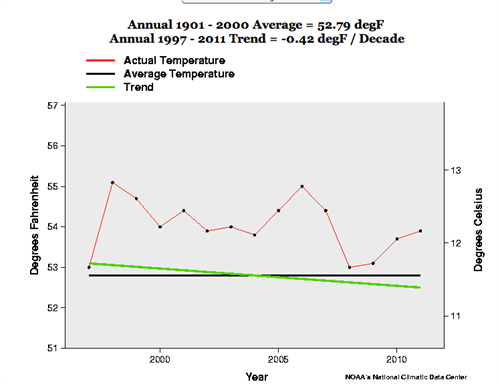
\includegraphics[width=0.5\textwidth]{img/cherry-1.png}
\end{center}
John Coleman, cited by  Anthony Watts, cited by \href{https://tamino.wordpress.com/2013/03/04/cherry-picking-is-childs-play/}{Open Mind}
\end{frame}

\begin{frame}{Not if you zoom out}

\begin{center}
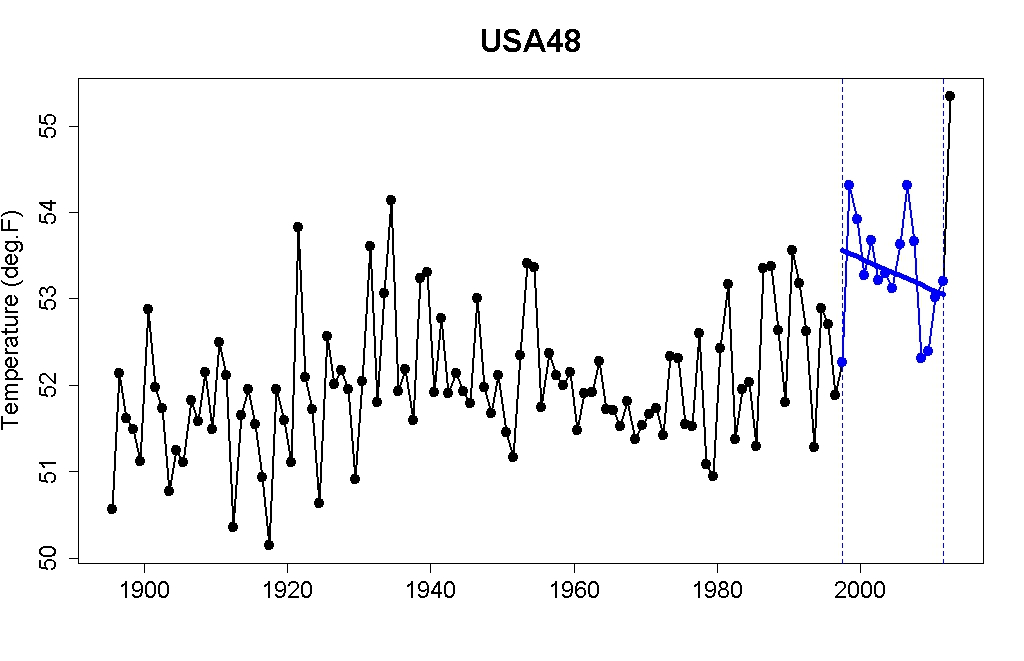
\includegraphics[width=0.6\textwidth]{img/usa48_1.jpg}
\end{center}
\href{https://tamino.wordpress.com/2013/03/04/cherry-picking-is-childs-play/}{Open Mind} \textit{Cherry Picking is Child's Play}
\end{frame}

\begin{frame}{And average over different regions}

\begin{center}
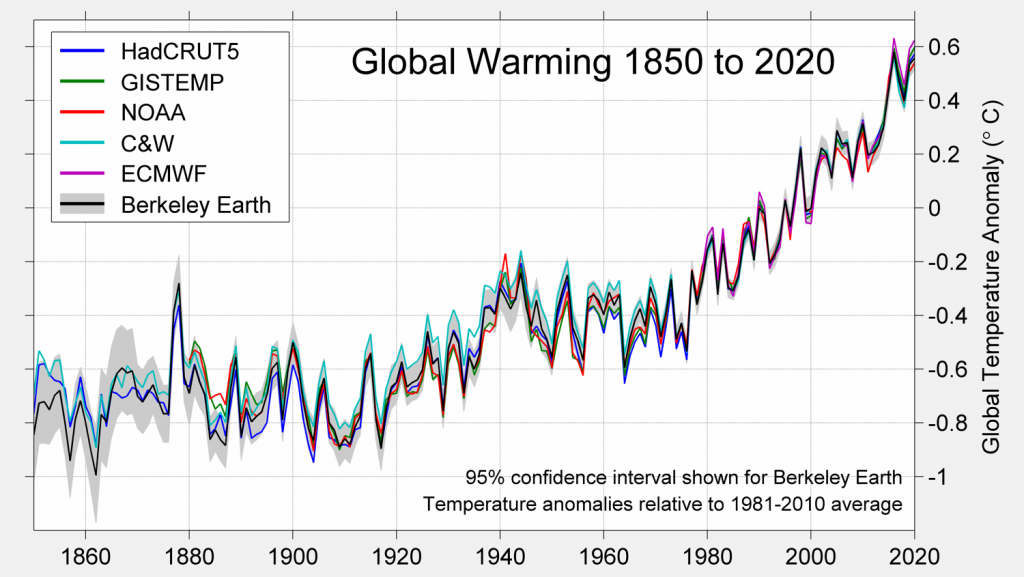
\includegraphics[width=0.6\textwidth]{img/1611534261_comparison-of-global-warming-trend-from-six-different-datasetspng.png}
\end{center}
\href{https://www.climate.gov.ph/news/416}{Climate Change Commission} \textit{CCC: No more time for inaction as global warming accelerates, marking 2020 as one of the warmest years on record} (graph: Berkeley Earth)
\end{frame}


% --- CHERRY-PICKING EXAMPLE
\begin{frame}{Example: cherry-picking data}
\textbf{What was done wrong?}
\begin{itemize}
  \item Only the years supporting the argument were shown
  \item Broader data contradicts the claimed trend
  \item No context or uncertainty provided
\end{itemize}
\textbf{Better practice:}
\begin{itemize}
  \item Show full dataset and acknowledge anomalies
  \item Explain the anomalies
  \item Show confidence intervals (the grey band in the last image)
  \end{itemize}

 If someone cherry picks data, and refuses to acknowledge it after it has been pointed out, then they are not a credible source\ldots

\end{frame}

% --- GRAPHICAL DECEPTION
\begin{frame}{How (not) to lie with graphs}
\begin{itemize}
  \item \textbf{Truncated axes} exaggerate small changes
  \item \textbf{Omitted error bars} hide uncertainty
  \item \textbf{3D charts} distort visual proportions
  \item \textbf{Unequal scales} misrepresent relationships
\end{itemize}
\begin{center}
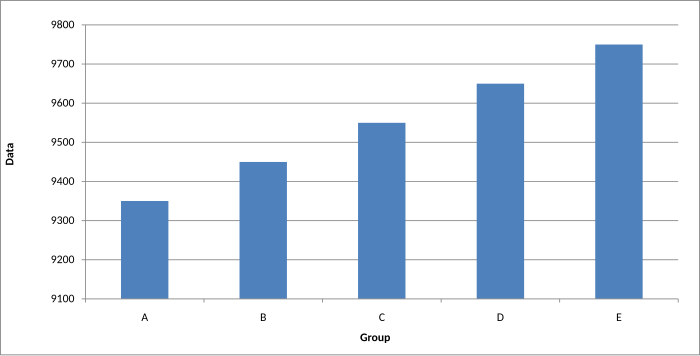
\includegraphics[width=0.4\textwidth]{img/700px-Truncated_Bar_Graph.svg.png}
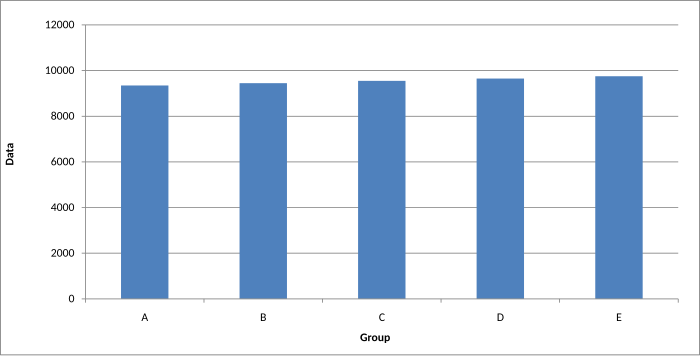
\includegraphics[width=0.4\textwidth]{img/700px-Bar_graph.svg.png}
\end{center}
Images from \href{https://en.wikipedia.org/wiki/Misleading_graph}{Wikipedia: Misleading graph} (CC BY-SA; accessed 2026-09-20)
\end{frame}

% --- FROM DATA TO ARGUMENT
\begin{frame}{From data to argument}
\begin{itemize}
  \item \textbf{FAIR failures} (missing metadata, unclear methods) give weak or unverifiable claims
  \item \textbf{CARE failures} (ignoring context or consent) give distorted or harmful stories
  \item So before you cite:
    \begin{itemize}
      \item Check where the data came from and how good it is
      \item Say how sure you are
      \item Describe people and communities the way they would recognise
    \end{itemize}
  \item This is as true for citing writing as it is for citing data!
\end{itemize}

\end{frame}

% =========================
% When Results Surprise You
% =========================

\section{When Results Surprise You}

% --- INTRODUCTION
\begin{frame}{When what you find surprises you}
\begin{itemize}
  \item You hypothesised X, and the data support Y, or nothing at all
  \item That is how discovery happens
  \item Many good findings began as ``wrong'' results someone looked into instead of hiding
  \item Report what you found, not what you hoped to find
\end{itemize}
If you discover that what you thought was wrong, \emph{then you have improved your model of the world}; if you just confirm what you thought, you have gained less!
\end{frame}

% --- ETHICAL RESPONSE
\begin{frame}{Ethical responses to unexpected results}
\begin{itemize}
  \item \textbf{Reflect}: why might this have happened? Re-check assumptions, methods, definitions
  \item \textbf{Consider alternatives}: sampling, measurement, confounders?
  \item \textbf{Report}: write down what changed in methods, data or interpretation
  \item \textbf{Revise}: update the theory to fit the evidence, not the other way round
\end{itemize}
\end{frame}

% --- FAIR + CARE CONNECTION
\begin{frame}{FAIR + CARE: supporting honest revision}
\begin{itemize}
  \item \txx{FAIR} (metadata, versioning, provenance) lets others trace how a result emerged
  \item \txx{CARE} (context, consent, responsibility) says how to interpret a surprise about people
  \item Complete records let you, and others:
    \begin{itemize}
      \item Reanalyse the same dataset later
      \item Identify methodological errors
      \item Reuse data collected by others, with its context
    \end{itemize}
  \item This applies to found data too: when you reuse an open dataset, respect its limits and write down your reasoning
\end{itemize}

\end{frame}

% =========================
% Writing Styles: Science, Creativity, Wikipedia
% =========================

\section{Writing for Different Audiences}

% --- COMPARISON OVERVIEW
\begin{frame}{Scientific, creative, and encyclopedic writing}
\begin{itemize}
  \item \txx{Scientific}: formal, objective, structured
    \begin{itemize}
      \item Evidence-based, peer-reviewed, reproducible
      \item Goal: to inform and test ideas transparently
    \end{itemize}
  \item \txx{Creative}: expressive, narrative, open to emotion and metaphor
    \begin{itemize}
      \item Goal: to move, provoke, or entertain
      \item Its truth is emotional or imaginative
    \end{itemize}
  \item \txx{Wikipedia}: concise, neutral, verifiable
    \begin{itemize}
      \item Summarises the consensus; takes no side
      \item Accessible to a broad, multilingual audience
    \end{itemize}
\end{itemize}

\end{frame}

% =========================
% Ethics in Fiction Writing (with citations)
% =========================
\subsection{Ethics in Fiction Writing}

% --- ETHICAL IMAGINATION
\begin{frame}{Ethical imagination}
\begin{itemize}
  \item Fiction is free to invent; does that freedom come with responsibility?
  \item Writers shape how readers see the world, other cultures, and themselves
  \item \txx{Ethical imagination}: invent without exploiting other people's pain or identity
  \item Ask:
    \begin{itemize}
      \item Whose stories am I telling?
      \item Do I have the right, or the context, to tell them?
      \item Who might be harmed or misrepresented by this portrayal?
    \end{itemize}
  \item Careless storytelling reinforces stereotypes; careful storytelling widens what readers can imagine
\end{itemize}

\medskip
\small Sources: \citep{hachette2021guidediversity, haynes2021ethicsaesthetics, leclerc2024writing}
\end{frame}

% --- CULTURAL SENSITIVITY AND RESPONSIBILITY
\begin{frame}{Cultural sensitivity and responsibility}
\begin{itemize}
  \item \txx{Cultural sensitivity} is awareness, and nobody is asking you to censor yourself
  \item Portray groups and traditions accurately, based on research and listening
  \item Avoid:
    \begin{itemize}
      \item Cultural elements as exotic decoration (appropriation)
      \item Reducing people to symbols or stereotypes
      \item Borrowing trauma without accountability
    \end{itemize}
  \item When writing outside your own experience:
    \begin{itemize}
      \item Consult people from that background
      \item Be open to feedback and revision
    \end{itemize}
\end{itemize}
\medskip
\small Sources: \citep{ocallaghan2025culturalsensitivity, maguire2009ethicsfiction, hachette2021guidediversity}

\begin{center}
\emph{I am not an expert here}
\end{center}

\end{frame}



% =========================
% Transition to Discussion / Activity
% =========================

\begin{frame}[allowframebreaks]{Acknowledgements}
  \small
  \begin{itemize}
  \item \textbf{Temperature graphs:} the two US 48-state plots come from
    Tamino's \href{https://tamino.wordpress.com/2013/03/04/cherry-picking-is-childs-play/}{Open Mind}
    post \textit{Cherry-Picking is Child's Play} (2013-03-04), which is
    rebutting John Coleman, reposted by Anthony Watts.  The six-dataset
    comparison is from
    \href{https://www.climate.gov.ph/news/416}{the Philippine Climate Change Commission},
    who credit Berkeley Earth.
  \item \textbf{Bar charts:} the truncated and untruncated bar graphs are from
    \href{https://en.wikipedia.org/wiki/Misleading_graph}{Wikipedia: Misleading graph} (CC BY-SA).
  \item \textbf{CARE material} draws on the Global Indigenous Data Alliance
    \citep{CARE2020}.
  \item \textbf{The AO3 case study} rests on the
    \href{https://archiveofourown.org/}{Archive of Our Own} and the
    Organization for Transformative Works, including their statement on
    \href{https://www.transformativeworks.org/ai-and-data-scraping-on-the-archive/}{AI and data scraping on the Archive}.
  \item \textbf{AI disclosure:} \textbf{GPT-4o} in ChatGPT
    \citep{openai-chatgpt-2025-03-14} was used to format the references and
    to draft an early version of these slides.
  \aicheck
  \end{itemize}
\end{frame}


% ====================================================
\begin{frame}[allowframebreaks]
\frametitle{References}
\printbibliography[heading=none]
\end{frame}


\end{document}
%%% Local Variables:
%%% coding: utf-8
%%% mode: latex
%%% TeX-engine: luatex
%%% End:
